\part{How programs are executed}
\frame{\partpage}

\begin{frame}{Executing programs}
    \begin{itemize}
        \item CPUs execute \textbf{machine code} \pause
        \item Programs must be \textbf{translated} into machine code for execution \pause
        \item There are three main ways of doing this: \pause
        \begin{itemize}
            \item An \textbf{interpreter} is an application which reads the program source code and executes it directly \pause
            \item An \textbf{ahead-of-time (AOT) compiler}, often just called a \textbf{compiler},
							is an application which converts the program source code into executable machine code \pause
            \item A \textbf{just-in-time (JIT) compiler} is halfway between the two --- it compiles the program on-the-fly
                at runtime
        \end{itemize}
    \end{itemize}
\end{frame}

\begin{frame}{Examples}
	\begin{columns}[t,onlytextwidth]
		\begin{column}{0.3\textwidth}
		    Interpreted:
		    \begin{itemize}
		        \item Python
		        \item Lua
						\item JavaScript (in old web browsers)
		        \item Bespoke scripting languages
		    \end{itemize}
		\end{column} \pause
		\begin{column}{0.3\textwidth}
		    Compiled:
		    \begin{itemize}
		        \item C
		        \item C++
		        \item Swift
		    \end{itemize}
		\end{column} \pause
		\begin{column}{0.3\textwidth}
		    JIT compiled:
		    \begin{itemize}
		        \item Java
		        \item C\#
		        \item JavaScript (in modern web browsers)
		        \item Jython
		    \end{itemize}
		\end{column}
	\end{columns}
	\pause NB: technically any language could appear in any column here, but this is where they typically are
\end{frame}

\begin{frame}{Interpreter vs compiler}
    \begin{itemize}
        \item Run-time efficiency: compiler $>$ interpreter \pause
        \begin{itemize}
            \item The compiler translates the program \textbf{in advance}, on the developer's machine \pause
            \item The interpreter translates the program \textbf{at runtime}, on the user's machine --- this takes extra time
        \end{itemize}
    \end{itemize}
\end{frame}

\begin{frame}{Interpreter vs compiler}
    \begin{itemize}
        \item Portability: compiler $<$ interpreter \pause
        \begin{itemize}
            \item A compiled program can only run on the operating system and CPU architecture it was compiled for \pause
            \item An interpreted program can run on any machine, as long as a suitable interpreter is available
        \end{itemize}
    \end{itemize}
\end{frame}

\begin{frame}{Interpreter vs compiler}
    \begin{itemize}
        \item Ease of development: compiler $<$ interpreter \pause
        \begin{itemize}
            \item Writing an AOT or JIT compiler (especially a good one) is hard, and required in-depth knowledge of the target machine \pause
            \item Writing an interpreter is easy in comparison
        \end{itemize}
    \end{itemize}
\end{frame}

\begin{frame}{Interpreter vs compiler}
    \begin{itemize}
        \item Dynamic language features: compiler $<$ interpreter \pause
        \begin{itemize}
            \item The interpreter is already on the end user's machine, so programs can use it e.g.\ to dynamically generate and execute new code \pause
            \item The AOT compiler is not generally on the end user's machine, so this is more difficult
        \end{itemize}
    \end{itemize}
\end{frame}

\begin{frame}{Interpreter vs compiler}
    \begin{itemize}
        \pause\item JIT compilers have similar pros/cons to interpreters
					\begin{itemize}
						\pause\item Runtime efficiency: JIT $>$ interpreter (e.g.\ code inside a loop only needs to be translated once, then can be executed many times)
						\pause\item Ease of development: JIT $<$ interpreter
					\end{itemize}
    \end{itemize}
\end{frame}

\begin{frame}{Virtual machines}
	\begin{itemize}
		\pause\item Many modern interpreters and JIT compilers translate programs into \textbf{bytecode}
		\pause\item Bytecode is essentially machine code for a \textbf{virtual machine (VM)}
		\pause\item Translation from source code to bytecode can be done ahead of time
		\pause\item At runtime, translate the bytecode (by interpretation or JIT compilation) into machine code for the physical machine
		\pause\item E.g.\ a Java JAR file, a .NET executable, a Python .pyc or .pyo file
			all contain bytecode for their respective VMs
	\end{itemize}
\end{frame}

\begin{frame}{Assemblers}
	\begin{itemize}
		\pause\item \textbf{Assembly language} is designed to translate directly into machine code
		\pause\item An ahead-of-time compile for assembly language is called an \textbf{assembler}
		\pause\item Generally much simpler than an AOT compiler for a higher-level language
	\end{itemize}
\end{frame}

\begin{frame}[fragile]{The C++ build process}
    \textbf{Preprocessor} \pause
    \begin{itemize}
        \item Handles \textbf{header inclusion}, \textbf{macro expansion} and \textbf{conditional compilation} \pause
        \item Outputs modified C++ source code \pause				
    \end{itemize}
    \textbf{Compiler} \pause
    \begin{itemize}
        \item Translates each source file into an \textbf{object file} containing machine code \pause
        \item May be configured to \textbf{optimise} code (e.g.\ calculate constant values, expand inline functions,
					re-order instructions to take advantage of CPU architecture, etc.) \pause
    \end{itemize}
    \textbf{Linker} \pause
    \begin{itemize}
        \item Combines the object files together with any external libraries to produce an \textbf{executable}
            (on Windows, a .exe file)
    \end{itemize}
\end{frame}

\begin{frame}[fragile]{The C++ build process}
    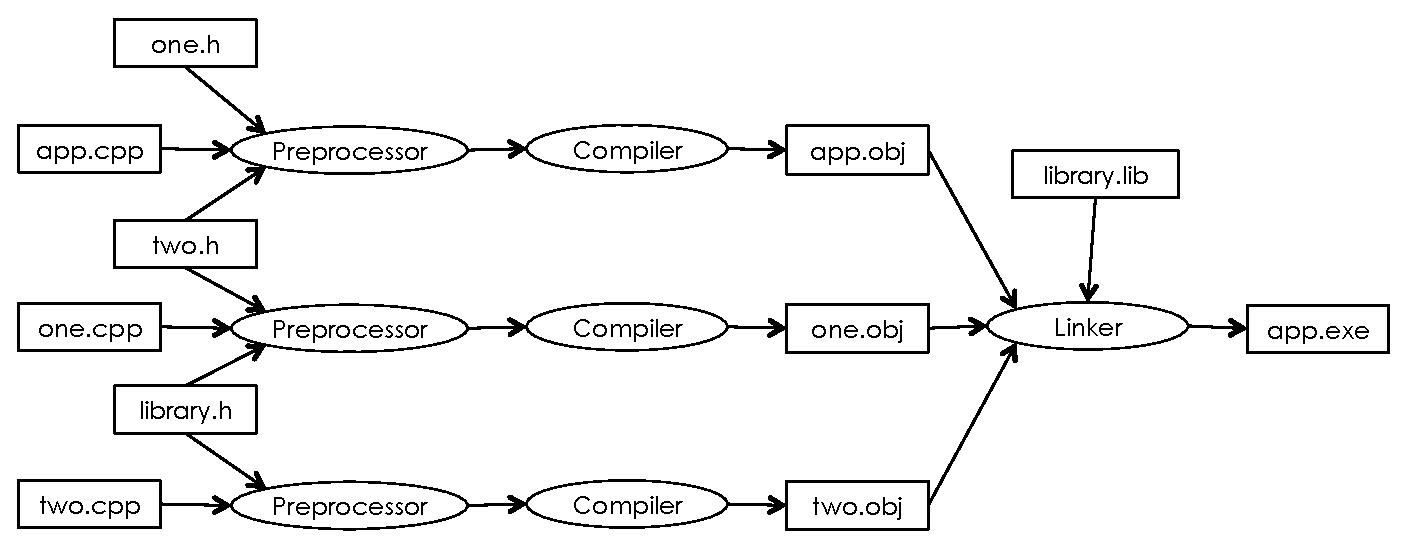
\includegraphics[width=\textwidth]{compiler_flowchart.pdf}
\end{frame}
